\documentclass[a4paper,12pt]{report}

\usepackage{graphicx}

\usepackage{enumitem}
\usepackage{lipsum}

\setlist[itemize]{leftmargin=*}

\setlength{\parindent}{0.0truein} % This will stop paragraphs indenting
\setlength{\textwidth}{17cm}
\setlength{\textheight}{24.25cm}
\setlength{\voffset}{-2cm}
\setlength{\hoffset}{-1.25cm}
\setlength{\parskip}{0.15truein} % This is the gap between paragraphs


\begin{document}

\newcommand{\beq}{\[}
\newcommand{\eeq}{\]}
\newcommand{\bneq}{\begin{equation}}
\newcommand{\eneq}{\end{equation}}
\newcommand{\bea}{\begin{eqnarray}}
\newcommand{\eea}{\end{eqnarray}}



\def\frameqn#1#2{\begin{center} \fbox{\parbox{#2}{\bneq #1 \eneq}} \end{center}}

\def\ltsima{$\; \buildrel < \over \sim \;$}
\def\simlt{\lower.5ex\hbox{\ltsima}}
\def\gtsima{$\; \buildrel > \over \sim \;$}
\def\simgt{\lower.5ex\hbox{\gtsima}}

\newsavebox{\savepar}
\newenvironment{boxit}{\begin{lrbox}{\savepar}
\begin{minipage}[b]{15.8cm}}
{\end{minipage}\end{lrbox}\fbox{\usebox{\savepar}}}

\setcounter{chapter}{1}

{\small Max Pettini: The Origin of The Elements}

{\normalsize

\begin{center}
\textbf{THE ORIGIN OF THE ELEMENTS}
\end{center}

Lecturer: Max Pettini  (Institute of Astronomy, Cambridge)\\
(maxpettini@icloud.com; www.ast.cam.ac.uk/$\sim$pettini)

{\bf Learning objectives:}
\begin{itemize}
\item Big-Bang Nucleosynthesis.
\item Energy production in stars, hydrogen burning and catalytic cycles.
\item Helium Burning and the $\alpha$-elements.
\item Slow and rapid neutron capture.
\item Explosive nucleosynthesis.
\item The sites of nucleosynthesis.
\end{itemize}

\section{Abstract}
At the beginning of the Universe matter appeared as protons and
neutrons.  Early fusion could get as far as helium-4 but not beyond.
Everything else requires stars in which heavier elements might be
considered as nuclear waste products.  Main-sequence stars are fusing
hydrogen to helium either directly or by catalytic cycles.  Once
hydrogen has been exhausted and the temperature has risen sufficiently
helium nuclei can fuse to form carbon, oxygen, neon etc., the $\alpha$
elements.  Beyond the iron group fusion no longer releases energy and
heavier elements require capture of uncharged neutrons.  We examine
in which stars and when these processes proceed along with how the
enriched material is returned to the interstellar medium whence it can
be incorporated in new stars and planets.


\section{Big-Bang Nucleosynthesis}
The initial seeds of BBN were sown by George Gamow, his PhD student Ralph Alpher, and Robert Herman in the years after the Second World War. These physicists realised that in the early 
stages of the universe expansion---`the first three minutes'---temperature and densities were sufficiently high to favour a number of nuclear reactions involving protons and neutrons leading to the synthesis of heavier elements up to $^7$Li,  as shown in Figure~\ref{fig:BBN}. 


 \begin{figure}[]
\setlength{\unitlength}{1.0cm}
\vspace*{-0.5cm}
\centerline{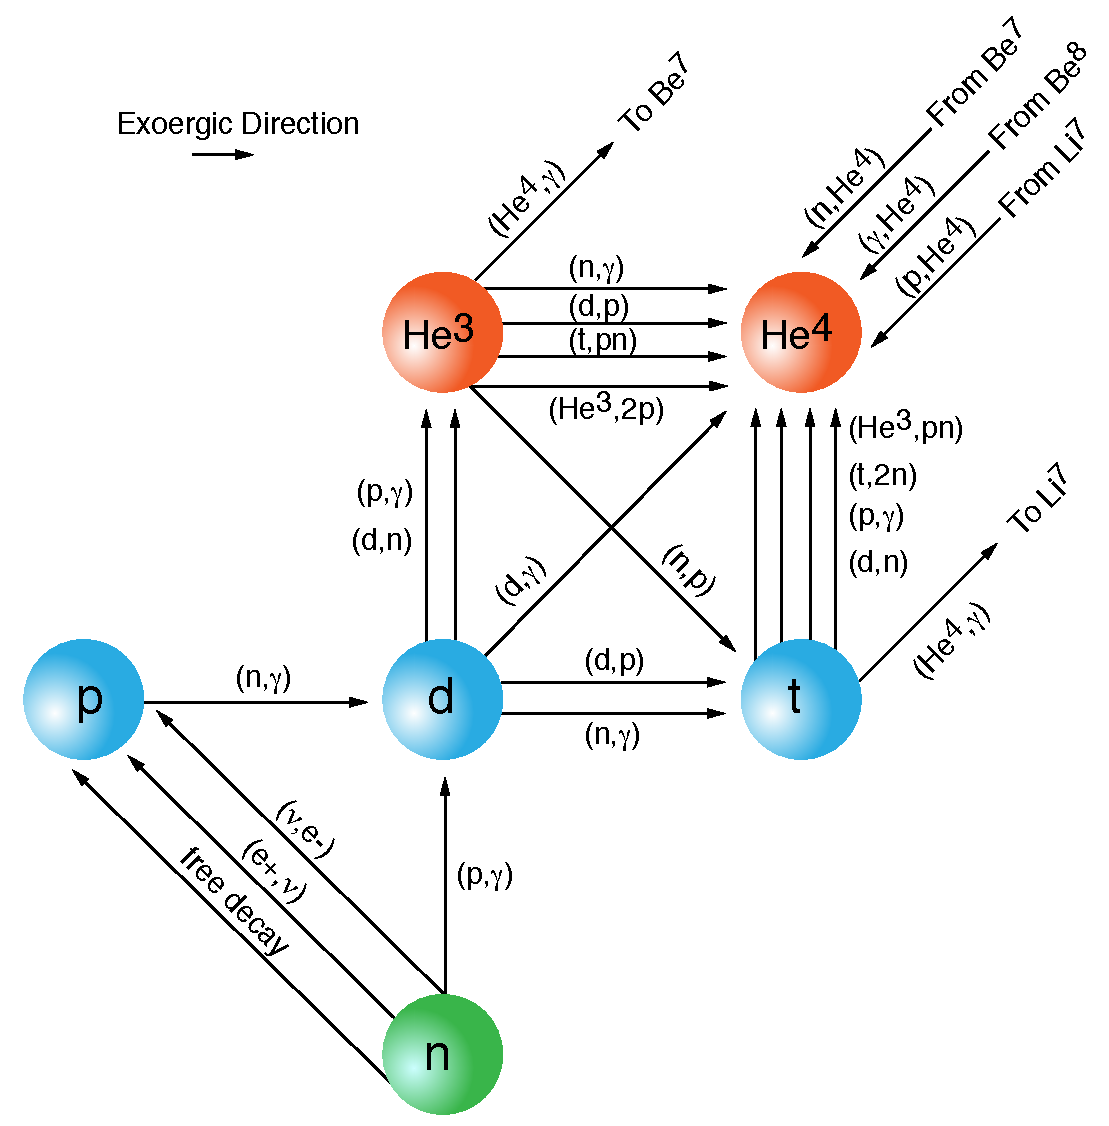
\includegraphics[width=10.95cm]{BigBang_network_HiRes_Cococubed}}
%\vspace{-0.75cm}
\caption{The network of reactions of primordial nucleosynthesis}
\medskip
\label{fig:BBN}
\end{figure}


All the other elements of the Periodic Table --- those that make astronomy, the natural world and life so interesting --- were either manufactured in the interior of stars or in the stars' final explosions. Mass loss from stars, either during or at the end of their lives, returns some of the products of \textit{stellar} nucleosynthesis to ambient medium, the interstellar medium of galaxies. Subsequent generations of stars---and their planets---form from this enriched interstellar medium in a cycle of galactic chemical evolution. As time progresses, galaxies, with their stars and planets, become progressively more enriched in chemical elements. In a confusing terminology, astronomers refer to ALL elements produced in stars as \textit{metals}, to distinguish them from the H and He made during BBN.

\section{How Do Stars Shine?}
Stars form in the cold, dense interiors of giant molecular clouds (GMCs): with infrared telescopes we see directly the process of star formation in such environments. Within GMCs, condensations with mass exceeding the so-called Jeans mass (which in turn depends on temperature and density) can easily come out of equilibrium and start collapsing under their own gravity. The collapse and subsequent accretion from the surroundings is halted once sufficient pressure is established in the core of the (proto-)star to balance in the inward pull of gravity. So, for a star to be in \textit{hydrostatic equilibrium} a \textit{negative pressure gradient} must exist within the star, with the pressure being larger in the
interior than near the surface:
\bneq
\frac{dP}{dr} = - \rho \, g \,, 
\label{eq:he3}
\eneq
where $P$ is the pressure, $\rho$ is the density and $g$ is the local acceleration of gravity at radius $r$.

What supplies the central pressure are nuclear reactions in the hot (millions of degrees) core of the star.
The simplest and most common nuclear reaction is the conversion of four protons (the nuclei of H) into a $^4$He nucleus.
To see how this works considers the following. 
If we wanted to break up a He nucleus (also sometime referred to 
as an alpha particle) into its constituents two protons and two neutrons,
we would need to supply $\sim 27$\,MeV.  It follows that
the inverse reaction, whereby four hydrogen nuclei fuse together
to form a He nucleus (plus a number of low mass remnants) will
release $\sim 27$\,MeV. This energy is the binding energy of
the He nucleus, and manifests itself as the mass difference between
four H nuclei (4.03 unified atomic mass units or 4.03\,u)
and one He nucleus (4.00\,u). 
This mass difference $\Delta m = 0.029$\,u,
or $\sim 0.7$\% of the rest mass of four  H nuclei,
corresponds to an energy $E = \Delta m \, c^2 = 26.7$\,MeV,
which is released by the nuclear fusion process.
This is fundamentally what powers the Sun and all life on Earth.

\section{Hydrogen Burning}
\subsection{The proton-proton chains}
The main reaction chain that powers stars during most of their lives is
hydrogen burning:
\beq
4 ^1_1\,{\rm H} \rightarrow \, ^4_2 \,{\rm He} + 2 e^+ + 2 \nu_e + 2 \gamma 
\eeq
which releases an energy  ${\cal E}_0 = 26.73$\,MeV. The two positrons subsequently annihilate
with free electrons: $e^+ \, + \, e^- = 2 \gamma$. The reaction can proceed 
through three channels (it is quite a common situation in nuclear reactions
that different pathways can lead to the same end result), as shown in 
Figure~\ref{fig:pp}. The balance between PP\,I and PP\,II varies
with temperature, with the former preferred at $T \simlt 1.5 \times 10^7$\,K;
the values indicated in Figure~\ref{fig:pp} are those appropriate
to the central temperature of the Sun, $T = 1.57 \times 10^7$\,K.
PP\,III is never very important, but it is a source of high energy
neutrinos.

\begin{figure}[b!]
\setlength{\unitlength}{1cm}
\vspace*{-0.5cm}
\centerline{\hspace*{-0.25cm}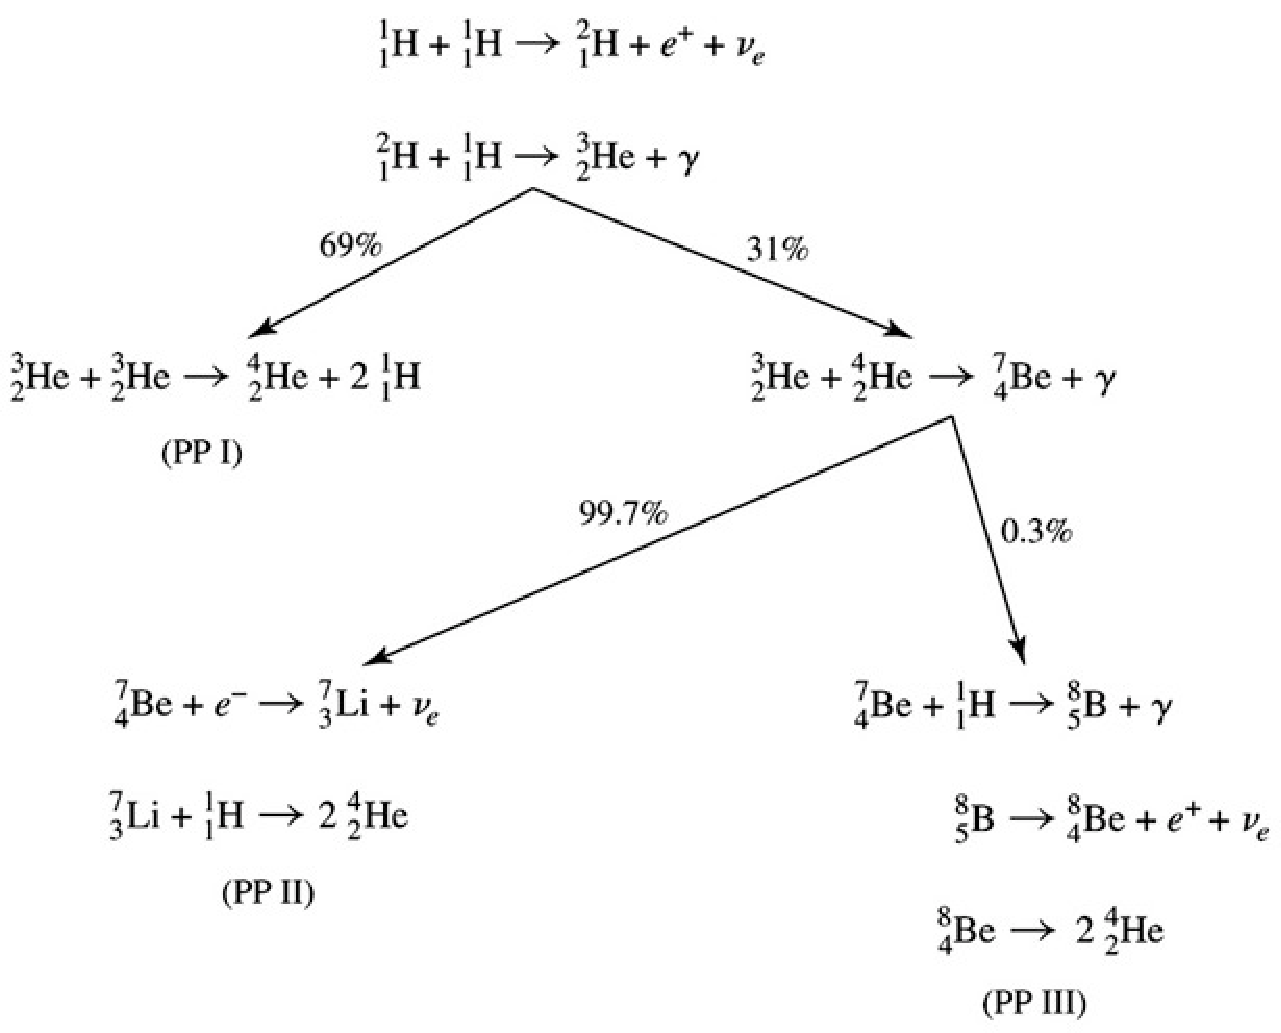
\includegraphics[width=8.9cm]{pp_chain1}}
%\vspace{-0.75cm}
\caption{The three proton-proton chains. The branching ratios are appropriate
to the temperature in the core of the Sun.}
%\medskip
\label{fig:pp}
\end{figure}

\subsection{The Carbon-Nitrogen-Oxygen cycle}
When C, N and O are present and the temperature is sufficiently
high, He can be synthesised from four H nuclei through a series
of pathways known as the CNO cycle.
C, N and O act as catalysts: they make He fusion possible through a
series of reactions, but their number is conserved in the cycle.
The two main pathways of the CNO cycle are as follows:\\

\centerline{\hspace*{-0.00025cm}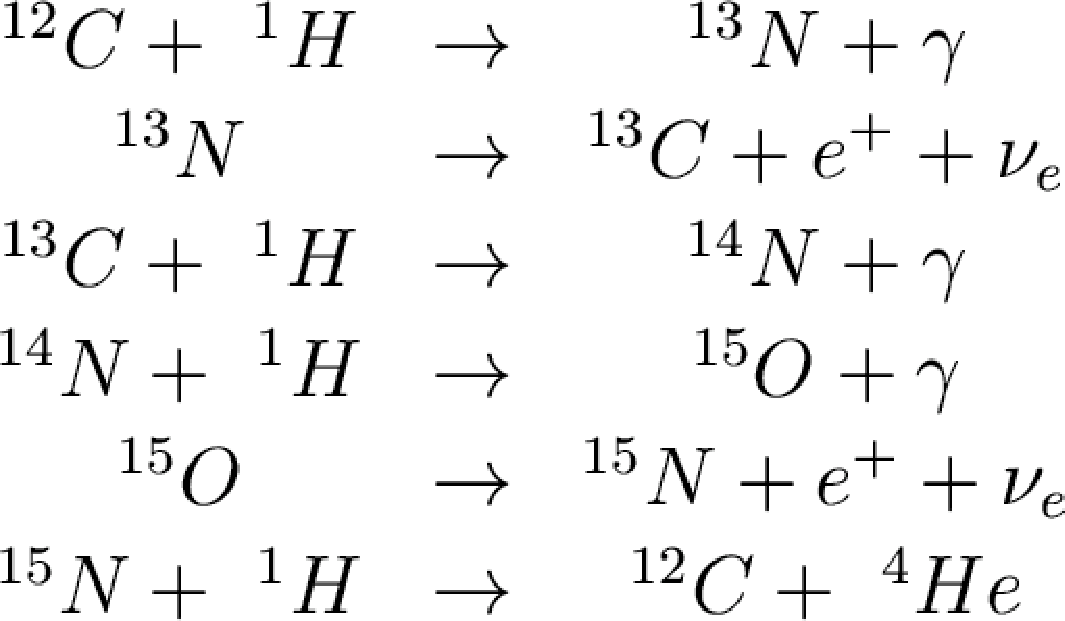
\includegraphics[width=6cm]{cno1}~~~~~~
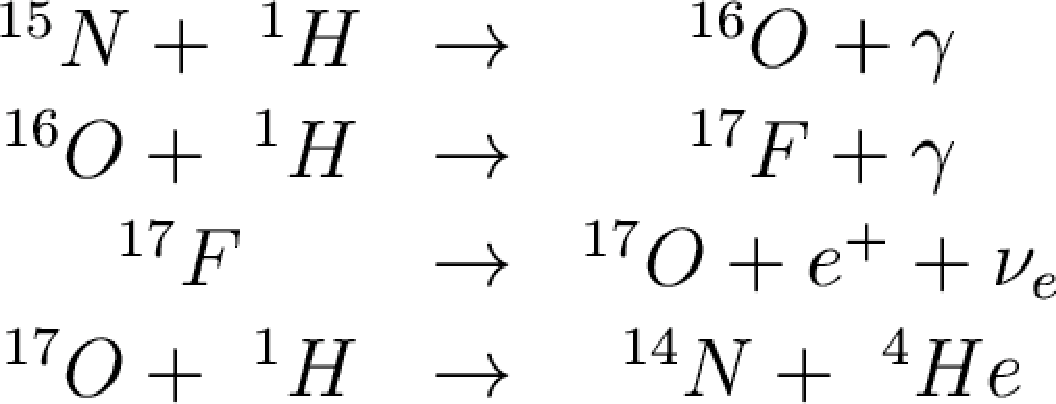
\includegraphics[width=6cm]{cno2}}

with the pathway on the right occurring only $\sim 0.04$\% of the time.
The proton capture by $^{14}$N is the slowest step in the cycle; consequently CNO elements 
tend to be converted to nitrogen during hydrogen burning.

The energy generation rates of both the p-p and CNO cycles are very sensitive to temperature: the higher the temperature, the higher the rate at which the nuclear reactions take place and therefore the more energy is released per second. The temperature dependences of the two processes are as follows:
\beq
{\cal E}_{\rm pp} \propto   T^4  ~~ {\rm and} ~~ {\cal E}_{\rm CNO} \propto   T^{17}  \,.
\eeq
The much steeper temperature dependence of the CNO cycle makes it the dominant energy production mechanism in massive stars, whose cores burn at temperatures in excess of 20 million degrees, while the p-p chain is favoured in lower mass stars, such as the Sun. The cross-over point is at $T \simeq 2 \times 10^7$\,K.

\begin{figure}[b!]
\setlength{\unitlength}{1cm}
\vspace*{-0.025cm}
\centerline{\hspace*{-0.25cm}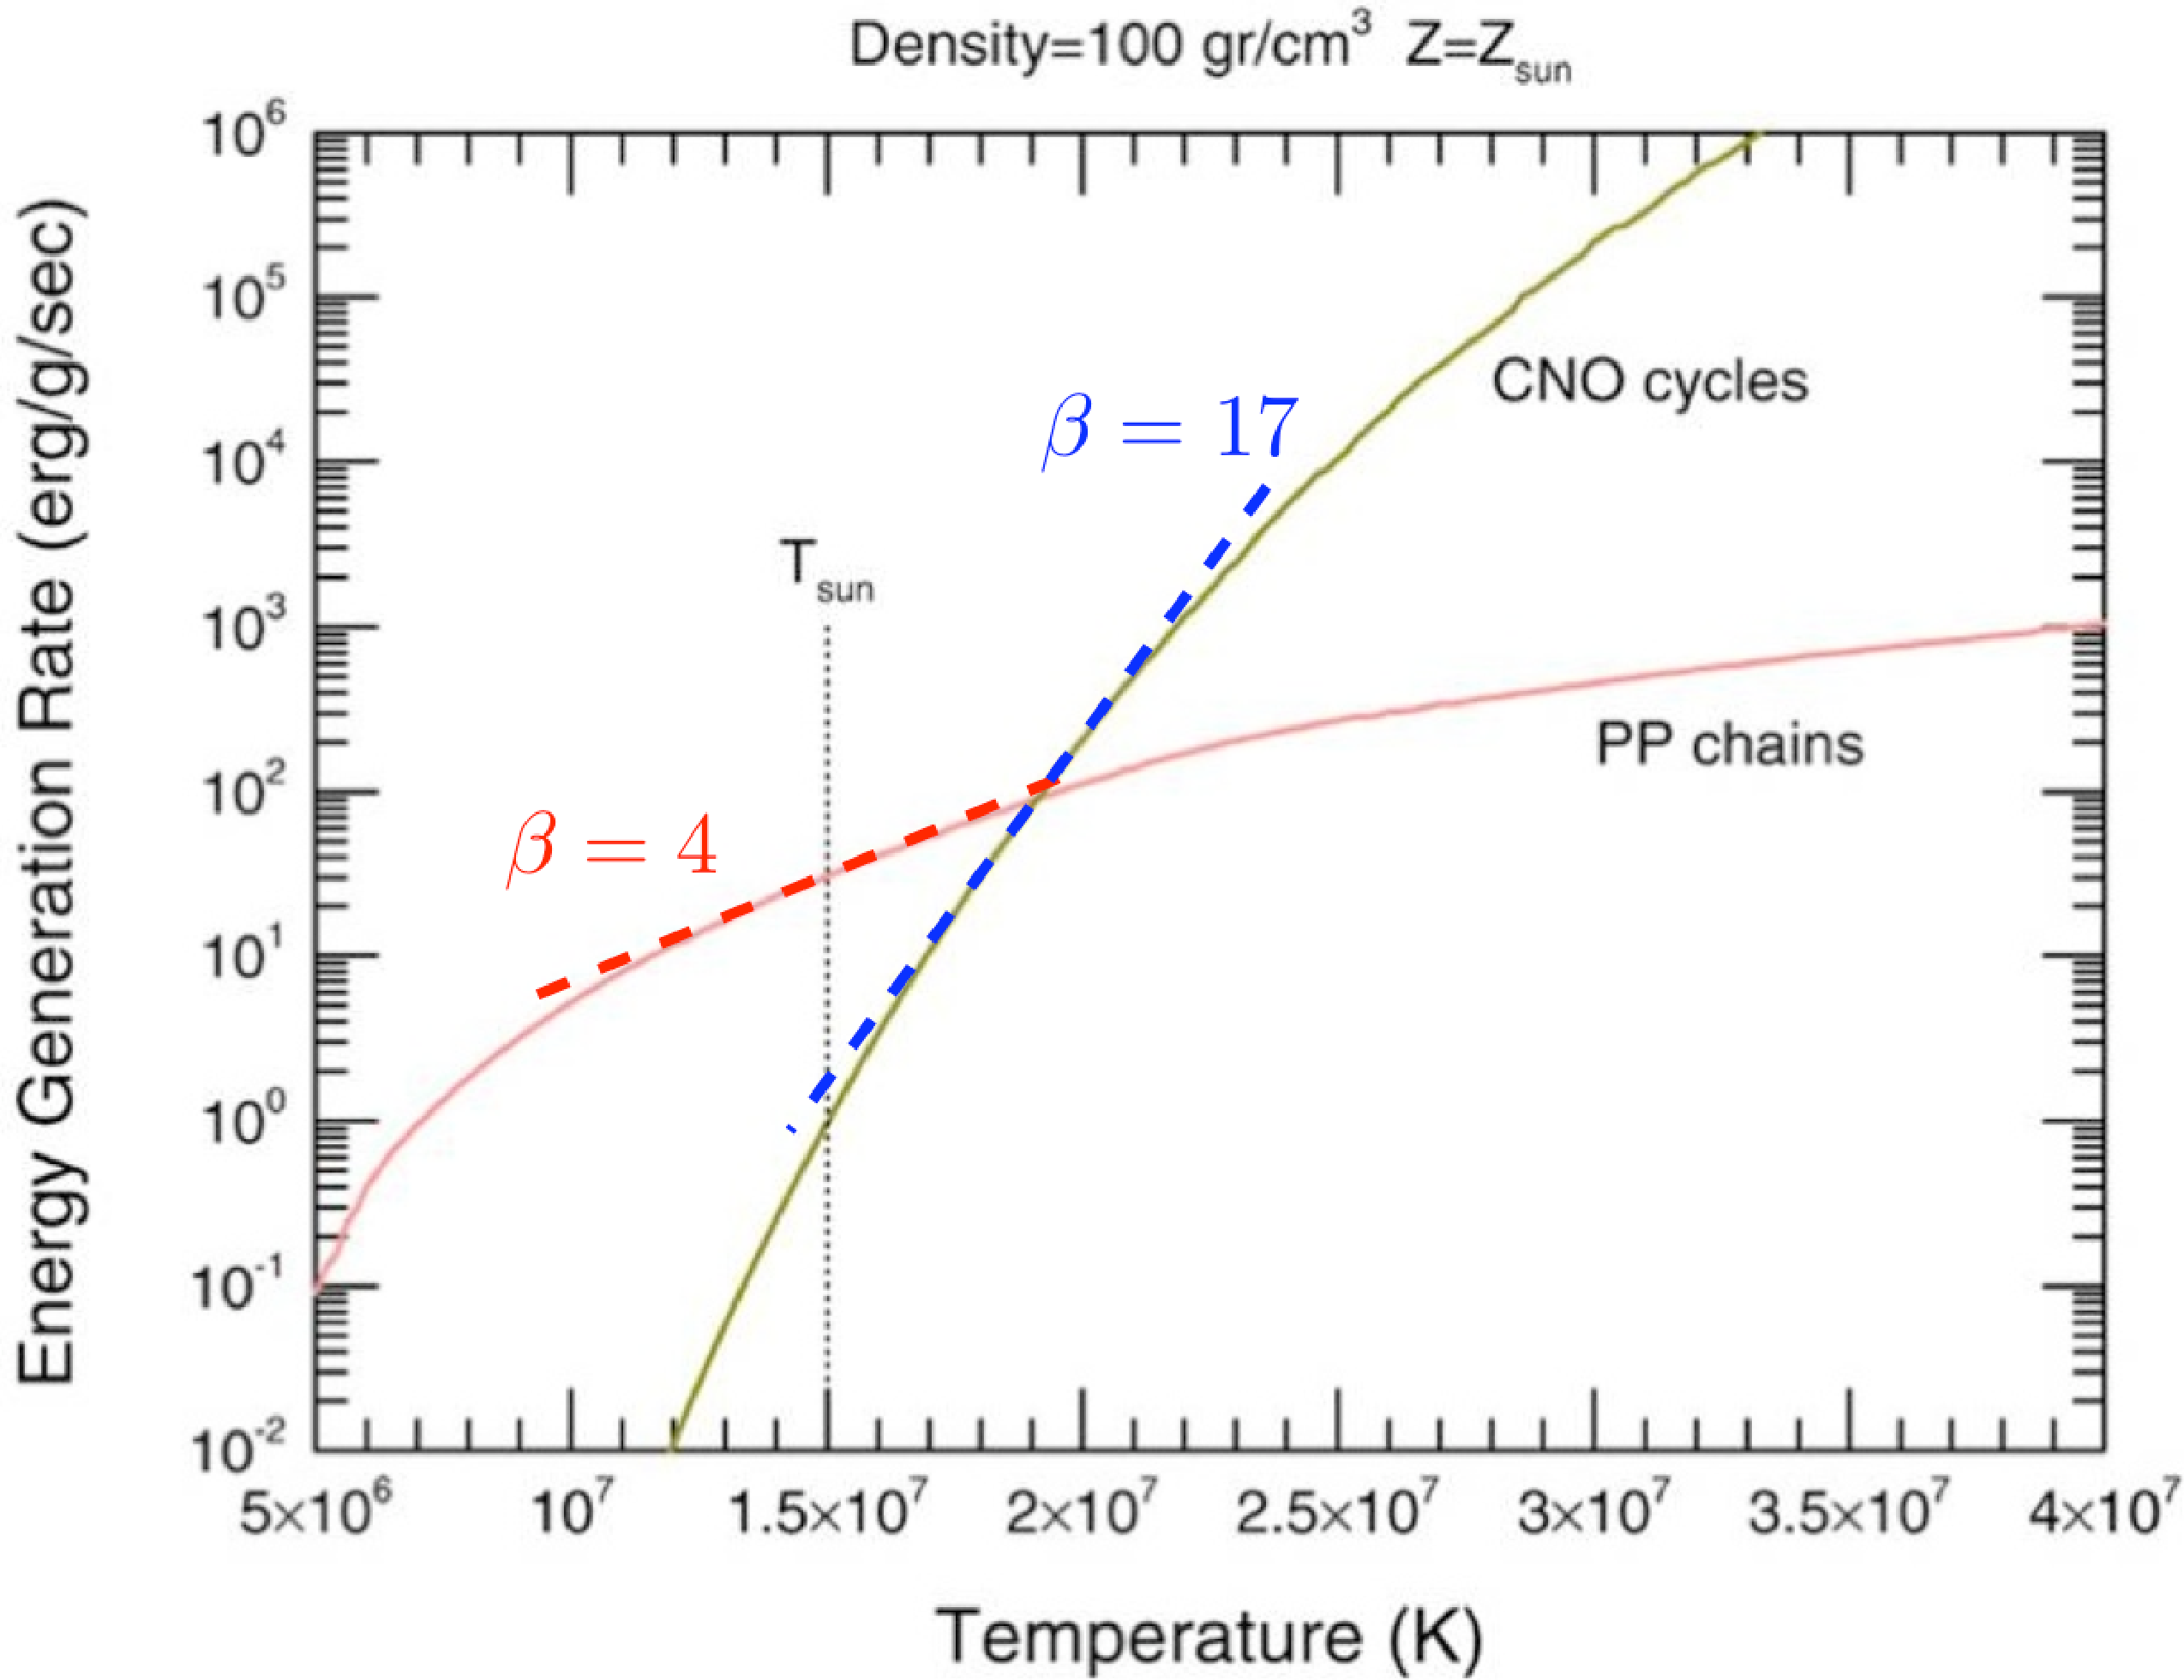
\includegraphics[width=10cm]{pp_CNO_T}}
\vspace{-0.025cm}
\caption{The temperature dependence of the energy generation rates
of the p-p chain and CNO cycle.}
%\medskip
\label{fig:pp_cno_T}
\end{figure}


At higher temperatures other catalytic cycles involving sodium, neon, magnesium can be activated.

\section{Helium Burning}
Whether it proceeds via the p-p chains or the CNO cycles, hydrogen burning leaves behind almost pure $^4$He
cores in stars. At that point the core contracts raising both the temperature and the density of the gas. 
When the temperature and density become sufficiently high ($T \approx 10^8$\,K), He nuclei---also referred to as alpha particles---can combine to form $^{12}$C by what is known as the triple-alpha process (see Figure~\ref{fig:3alpha})

\begin{figure}[h!]
\setlength{\unitlength}{1cm}
%\vspace*{-0.025cm}
\centerline{\hspace*{-0.25cm}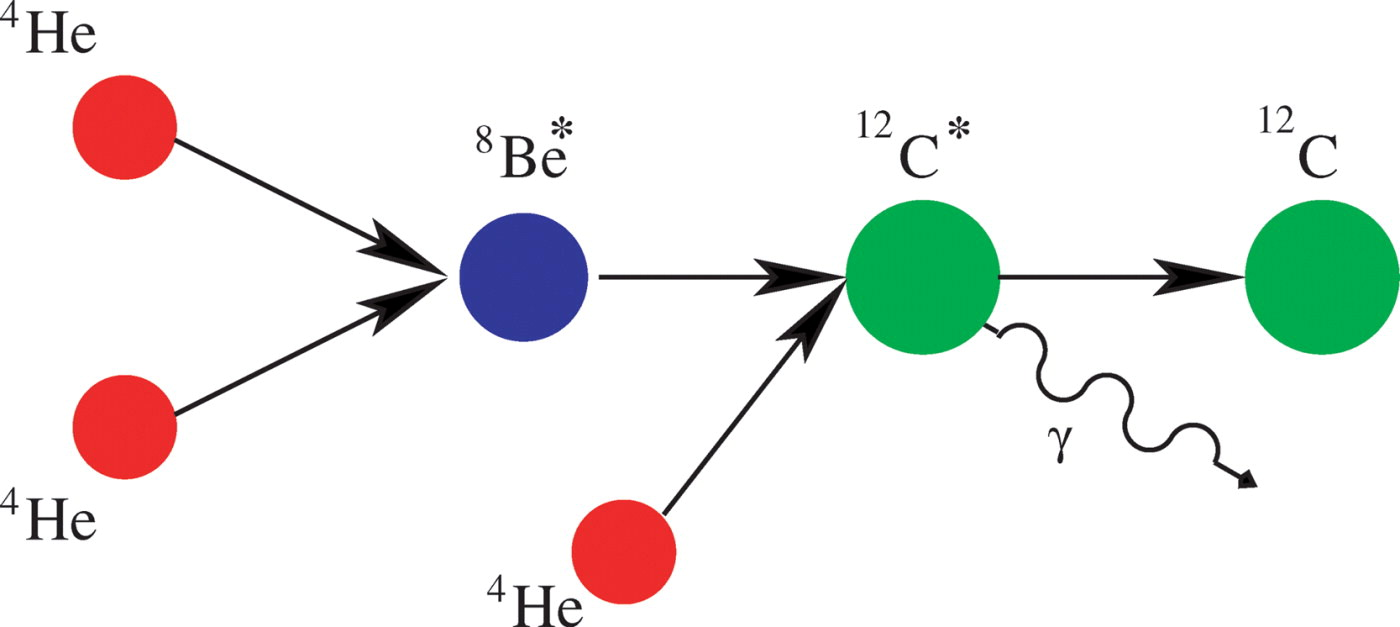
\includegraphics[width=11cm]{TripleAlpha_Tout}}
\vspace{0.15cm}
\caption{The triple-$\alpha$ process. Two $^4$He nuclei collide to form an unstable $^8$Be$^\ast$ nucleus. A third $^4$He nucleus collides with $^8$Be$^\ast$ before it breaks up to form the resonant excited $^{12}$C nucleus which loses energy to drop down to stable $^{12}$C.}
%\medskip
\label{fig:3alpha}
\end{figure}

This triple alpha reaction was predicted by Fred Hoyle (a previous
director of the Institute of Astronomy) in 1954, based on the high 
abundance of C in the Sun and H\,{\sc ii} regions like the
Orion nebula. It produces C from He nuclei bypassing completely
the intermediate elements Li, Be, B, and it explains why C is $10^5$--$10^7$
times more abundant that Li, Be and B in the Universe. 


\section{Advanced Burning Stages}
Once sufficient quantities of $^{12}$C have been synthesised via the
triple alpha reaction, heavier elements can be formed from $^{12}$C
via the capture of additional $^4$He nuclei:
\beq
^{12}_{~6}\,{\rm C} + ^4_2{\rm He}  \rightarrow ^{16}_{~8}{\rm O }+ \gamma
\eeq
\beq
^{16}_{~8}\,{\rm O} + ^4_2 {\rm He}\rightarrow ^{20}_{10}{\rm Ne} + \gamma
\eeq

\newpage 
Nitrogen that has accumulated during CNO hydrogen burning can also
capture an $\alpha$-particle:
\beq 
\rm {^{14}N} + {^4He} \rightarrow {^{18}F} + \gamma
\eeq
\beq
\rm {^{18}F} \rightarrow {^{18}O} + e^+ + \nu_{\rm e}
\eeq
\beq
\rm {^{18}O} + {^4He} \rightarrow {^{22}Ne} + \gamma
\eeq

\begin{figure}[]
\setlength{\unitlength}{1cm}
\vspace*{-0.25cm}
\centerline{\hspace*{-0.25cm}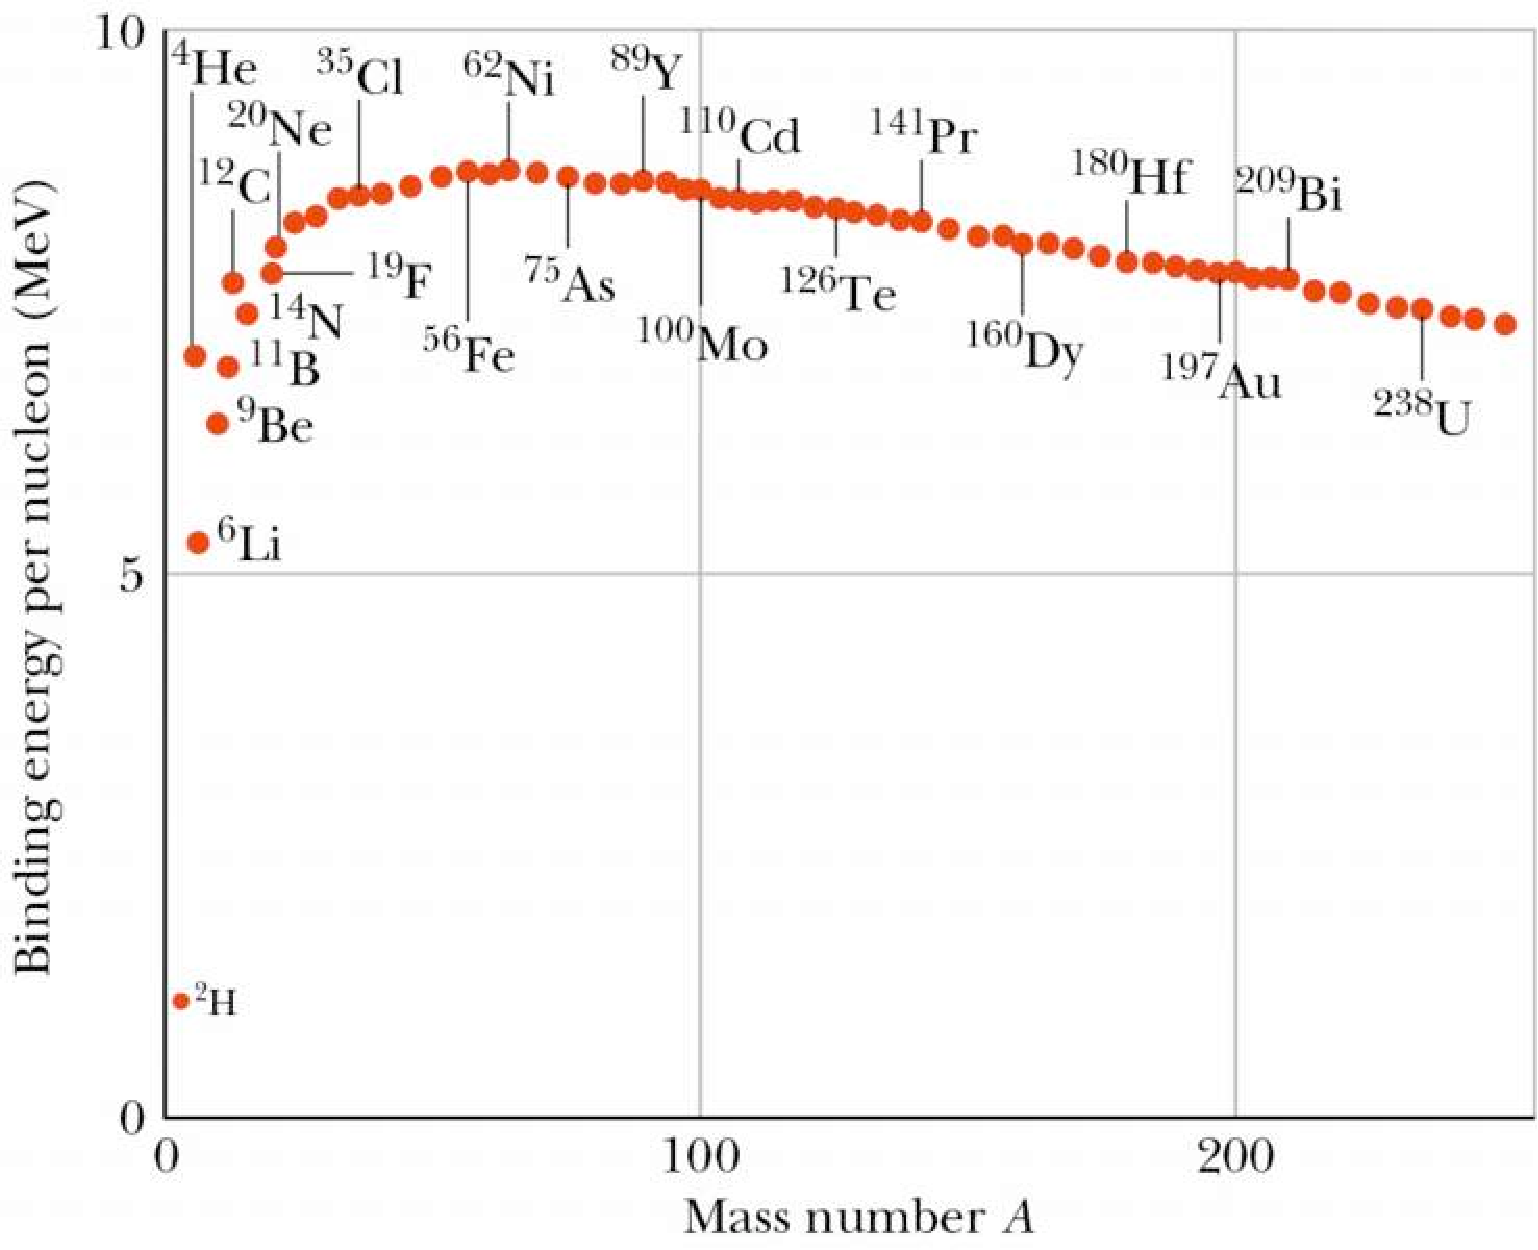
\includegraphics[width=7cm]{binding_energy_nuclei}~~~
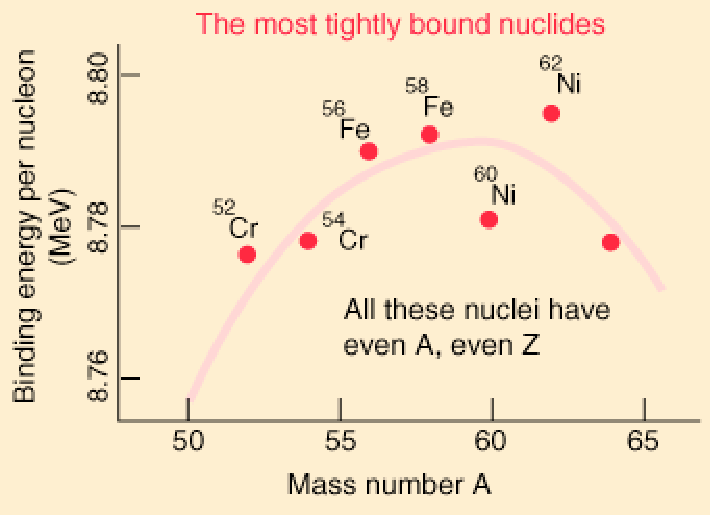
\includegraphics[width=7.7cm]{nucbint}
}
%\vspace{-0.25cm}
\caption{Left: Binding energy per nucleon as a function of mass number $A$. 
Right: Close-up near the iron peak. $^{62}_{28}$\,Ni has the highest binding energy 
per nucleon of any isotope of any element.
}
%\vspace{0.75cm}
\label{fig:bind_E}
\medskip
\end{figure}

As can be appreciated from Figure~\ref{fig:bind_E},
fusing elements beyond C releases progressively less energy per nucleon 
while requiring higher and higher temperatures to bring positively charged nuclei 
close enough for the fusion reactions to take place.
So each subsequent stage in the star's life last a progressively shorter time.
The process can continue so long as it is exothermic, that is so long
as the mean mass per nucleon of the final fusion product is lower than that
of the fusing nuclei. The binding energy per nucleon curve
(see Figure~\ref{fig:bind_E}) reaches a peak near Fe (hence the term
Fe-peak). Fusion of Fe-peak elements to form elements of higher mass
is an endothermic process requiring an additional supply of energy
(and conversely, energy can be released by the fission of these heavier
nuclei into lighter ones, as in a nuclear power station).

At the end of its life, the interior of a massive star is stratified, 
as shown in Figure~\ref{fig:onion_skin}. 
The formation of a core of iron-group elements marks the end of a star's
nuclear burning life.  When no more energy is available from
nuclear fusion to support the core, the core collapses
to a neutron star or a black hole.  The enormous release of
gravitational energy causes an explosion visible as
a core-collapse supernova which returns the processed outer layers to the
interstellar medium.

\begin{figure}[]
\setlength{\unitlength}{1cm}
\vspace*{-0.5cm}
\centerline{\hspace*{+0.25cm}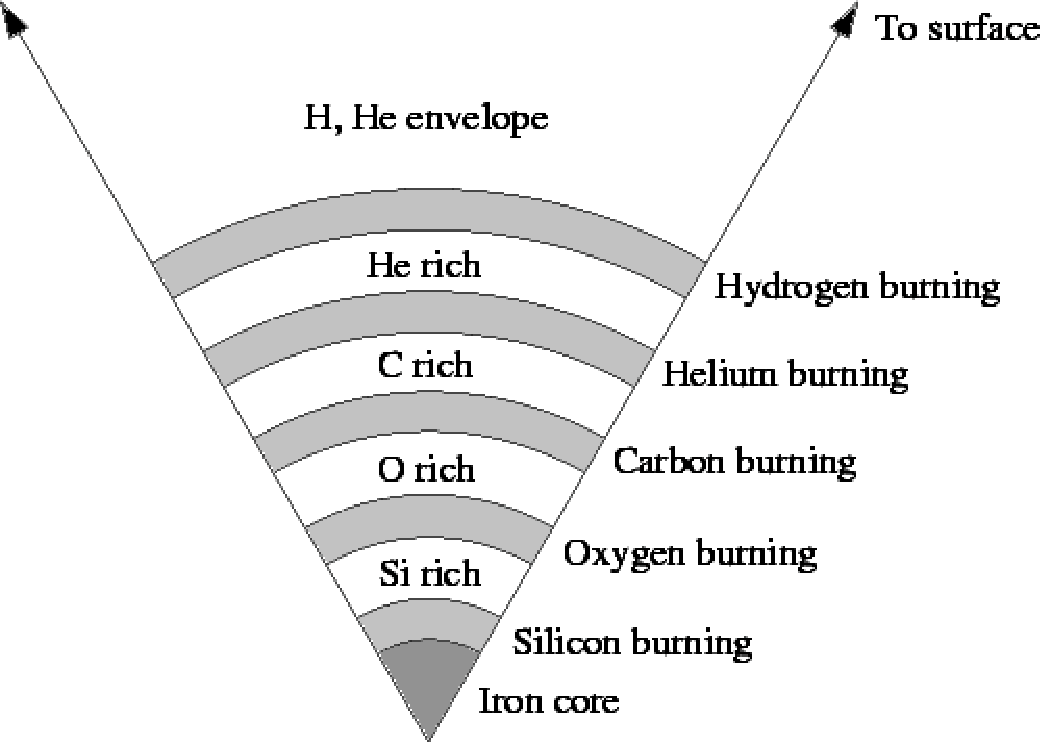
\includegraphics[width=8.75cm]{onion_skin1}}
%\vspace{-0.025cm}
\caption{The stratified structure of the core of a massive star.}
\medskip
\label{fig:onion_skin}
\end{figure}

\section{Iron and Type Ia Supernovae}
Most of the Iron synthesised by massive stars is not returned to the ISM, as it collapses into the neutron star or black hole. So where does Fe come from?

The origin is Fe is believed to be a different phenomenon which involves pairs of lower mass stars. Most stars are born in pairs (or more generally multiple systems). If the members of a binary pair are sufficiently close, mass can be transferred from one member to the other. Stars that start their lives with masses $M < 8 M_\odot$ never reach core temperatures high enough to burn C and O. At the end of their lives they eject their outer layers leaving behind a hot, compact CO core that slowly cools with time. Such a remnant is called a White Dwarf.

Quantum mechanics and special relativity tell us that there is a maximum mass for a WD, approximately $1.44\,M_\odot$,
called a Chandrasekhar mass after the Indian astronomer who first proposed this limit while working here in Cambridge.
If mass transfer onto a white dwarf results in this limit being exceeded, or if two binary white dwarfs merge, the star undergoes a thermonuclear explosion termed (for reasons that need not concern us here) a Type Ia supernova.
Just before the explosion, at about $1.38\,M_\odot$, cool carbon-oxygen white dwarfs reach densities at which cold carbon fusion begins, setting off a thermonuclear runaway in which most of the star reaches nuclear statistical equilibrium before entirely exploding. The end result is the production of about one solar mass of $^{56}$Ni which subsequently decays to $^{56}$Fe.

\section{Elements Heavier than Iron, Neutron Capture}
We conclude our description of stellar nucleosynthesis with a
brief mention of the mechanism whereby elements heavier than Fe are
thought to be produced in stars.

Neutrons have no electric charge and so no Coulomb barrier to overcome
when penetrating a nucleus.  They have very high reaction
cross-sections with nuclei that increase with the typical
area of the nucleus.
So neutrons are more easily captured by iron and heavier elements
than small light nuclei such as protons and $\alpha$-particles.  In
this way heavy, neutron-rich isotopes can be built up. 
Such isotopes can be either stable or unstable.


 \begin{figure}[t!]
\setlength{\unitlength}{1cm}
%\vspace*{-1.25cm}
\centerline{\hspace*{-0.15cm}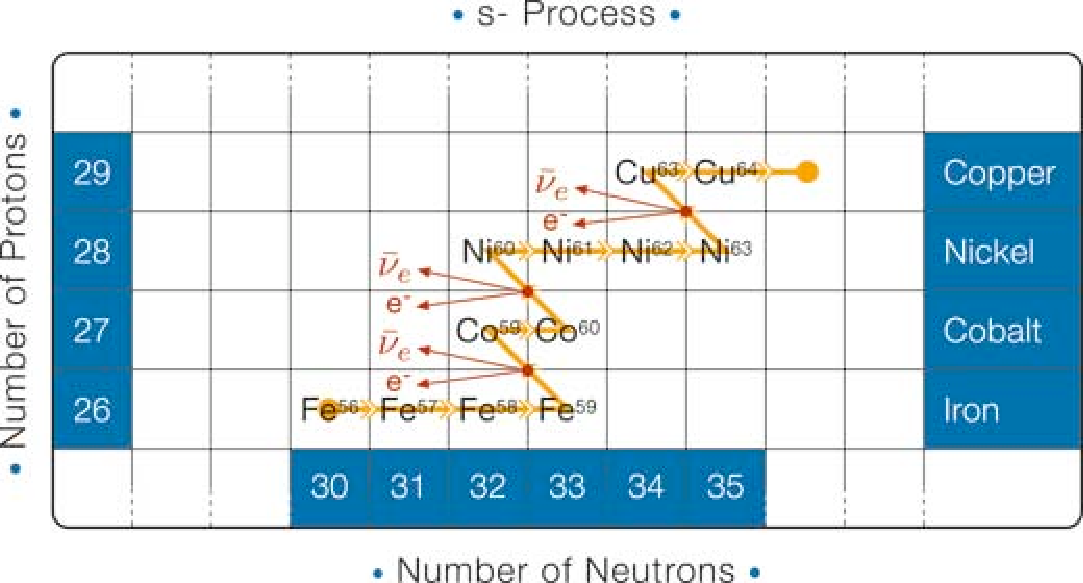
\includegraphics[width=11cm]{sprocess}}
%\vspace{-0.025cm}
\caption{Example of the nucleosynthesis of $^{59}$Co,   $^{60}$Ni and
$^{63}$Cu from $^{56}$Fe via slow neutron capture.
}
%\medskip
\label{fig:s-process}
\end{figure}

It is important to distinguish between slow and rapid neutron capture
(termed the s-process and the r-process), depending on the relative timescales
of $\beta$-decay and neutron capture. In the example of the s-process
shown in Figure~\ref{fig:s-process}, $^{56}$Fe absorbs a neutron to
form $^{57}$Fe. Subsequent capture of two more neutrons leads
to the formation of $^{59}$Fe. Of the four Fe isotopes shown, 
the three lighter ones are stable, but $^{59}$Fe is unstable,
with a half-life of 44.5 days. Thus, if the flux of neutrons is not high 
and the interval between successive n-captures is longer than 
the half-life of $^{59}$Fe, there is time for $^{59}$Fe to decay
to $^{59}$Co by $\beta$-decay (n\,$\rightarrow$\, p + e$^-$ + $\overline{\nu}_e$).
The process can continue to form higher and higher mass elements,
as shown in Figure~\ref{fig:s-process}.


 \begin{figure}[b!]
\setlength{\unitlength}{1cm}
%\vspace*{-0.25cm}
\centerline{\hspace*{-0.15cm}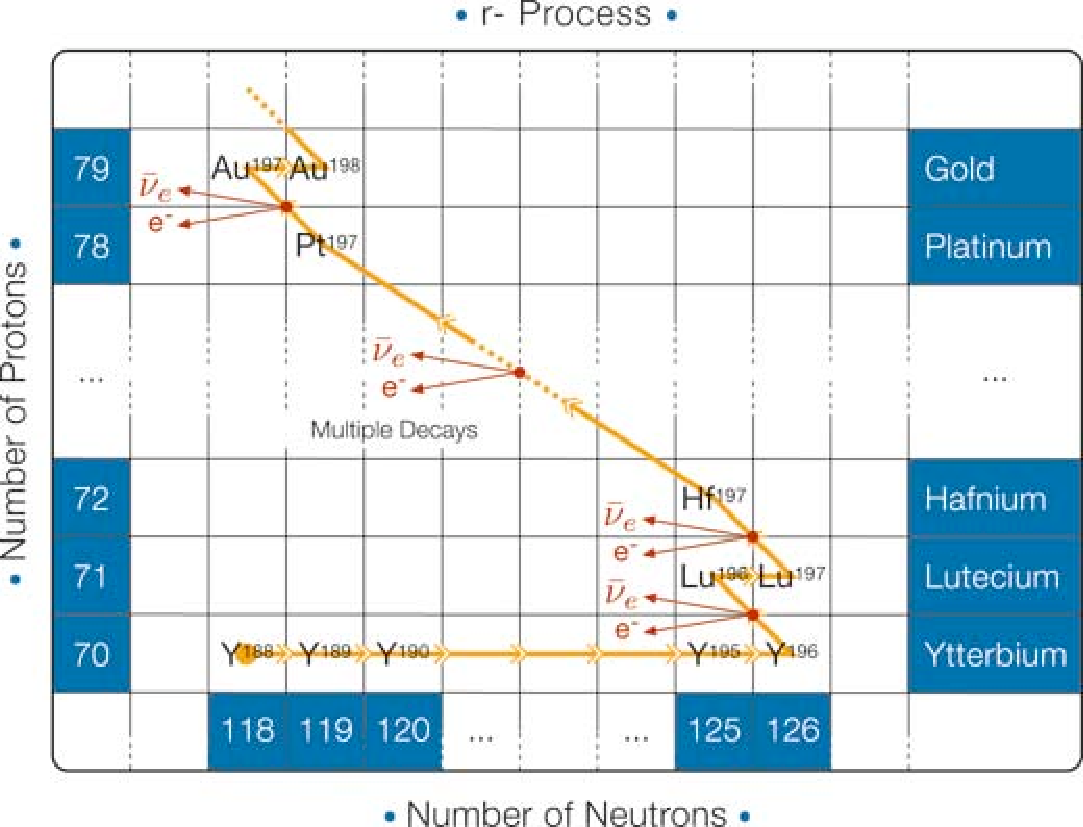
\includegraphics[width=8.75cm]{rprocess}}
%\vspace{-0.025cm}
\caption{Example of the nucleosynthesis of $^{197}$Au (stable gold) 
 from $^{188}$Yb via rapid neutron capture.
}
%\medskip
\label{fig:r-process}
\end{figure}

On the other hand, if the flux of neutrons is sufficiently high and the time interval
between subsequent neutron captures is small compared to the half-life
of the isotopes concerned, super-neutron-rich isotopes can be formed,
as in the example of the r-process shown in Figure~\ref{fig:r-process}.
When the neutron flux stops, these super-neutron-rich isotopes
will undergo a series of $\beta$-decays until a stable isotope is reached.

Trans-Fe-peak elements can be formed by either s- or r-process
nucleosynthesis, or both, depending on the stability of their neighbours
in the Periodic Table. 
Typical s-process elements include Cu and Pb, while Eu
is the prototypical signature of r-process nucleosynthesis in
stellar spectra.
It is generally though that s-process nucleosynthesis takes place
primarily in evolved low and intermediate mass stars, while the
r-process occurs mainly in supernova explosions
and, as now confirmed observationally, in 
the explosion accompanying the merger of two neutron stars.

\section{Conclusions}
Figure~\ref{fig:JJsPeriodicTable} collects together our ideas of the main sites and processes responsible for synthesising the elements of the Periodic Table.
Most elements beyond C and N and are produced in stellar explosions, whether the core-collapse of  massive stars, or the total disruption of lower mass stars in binary systems, or even the merging of neutron stars---an event only recently observed via the gravitational waves it generated. Supernovae and neutron star mergers are rare events within galaxies.  Evidently, there must be an efficient mechanism for distributing their seeds widely in the space between the stars so that they can be incorporated in subsequent generations of stars and planets, and finally make possible life on Earth and elsewhere.

 \begin{figure}[h!]
\setlength{\unitlength}{1cm}
\vspace*{0.75cm}
\centerline{\hspace*{-0.15cm}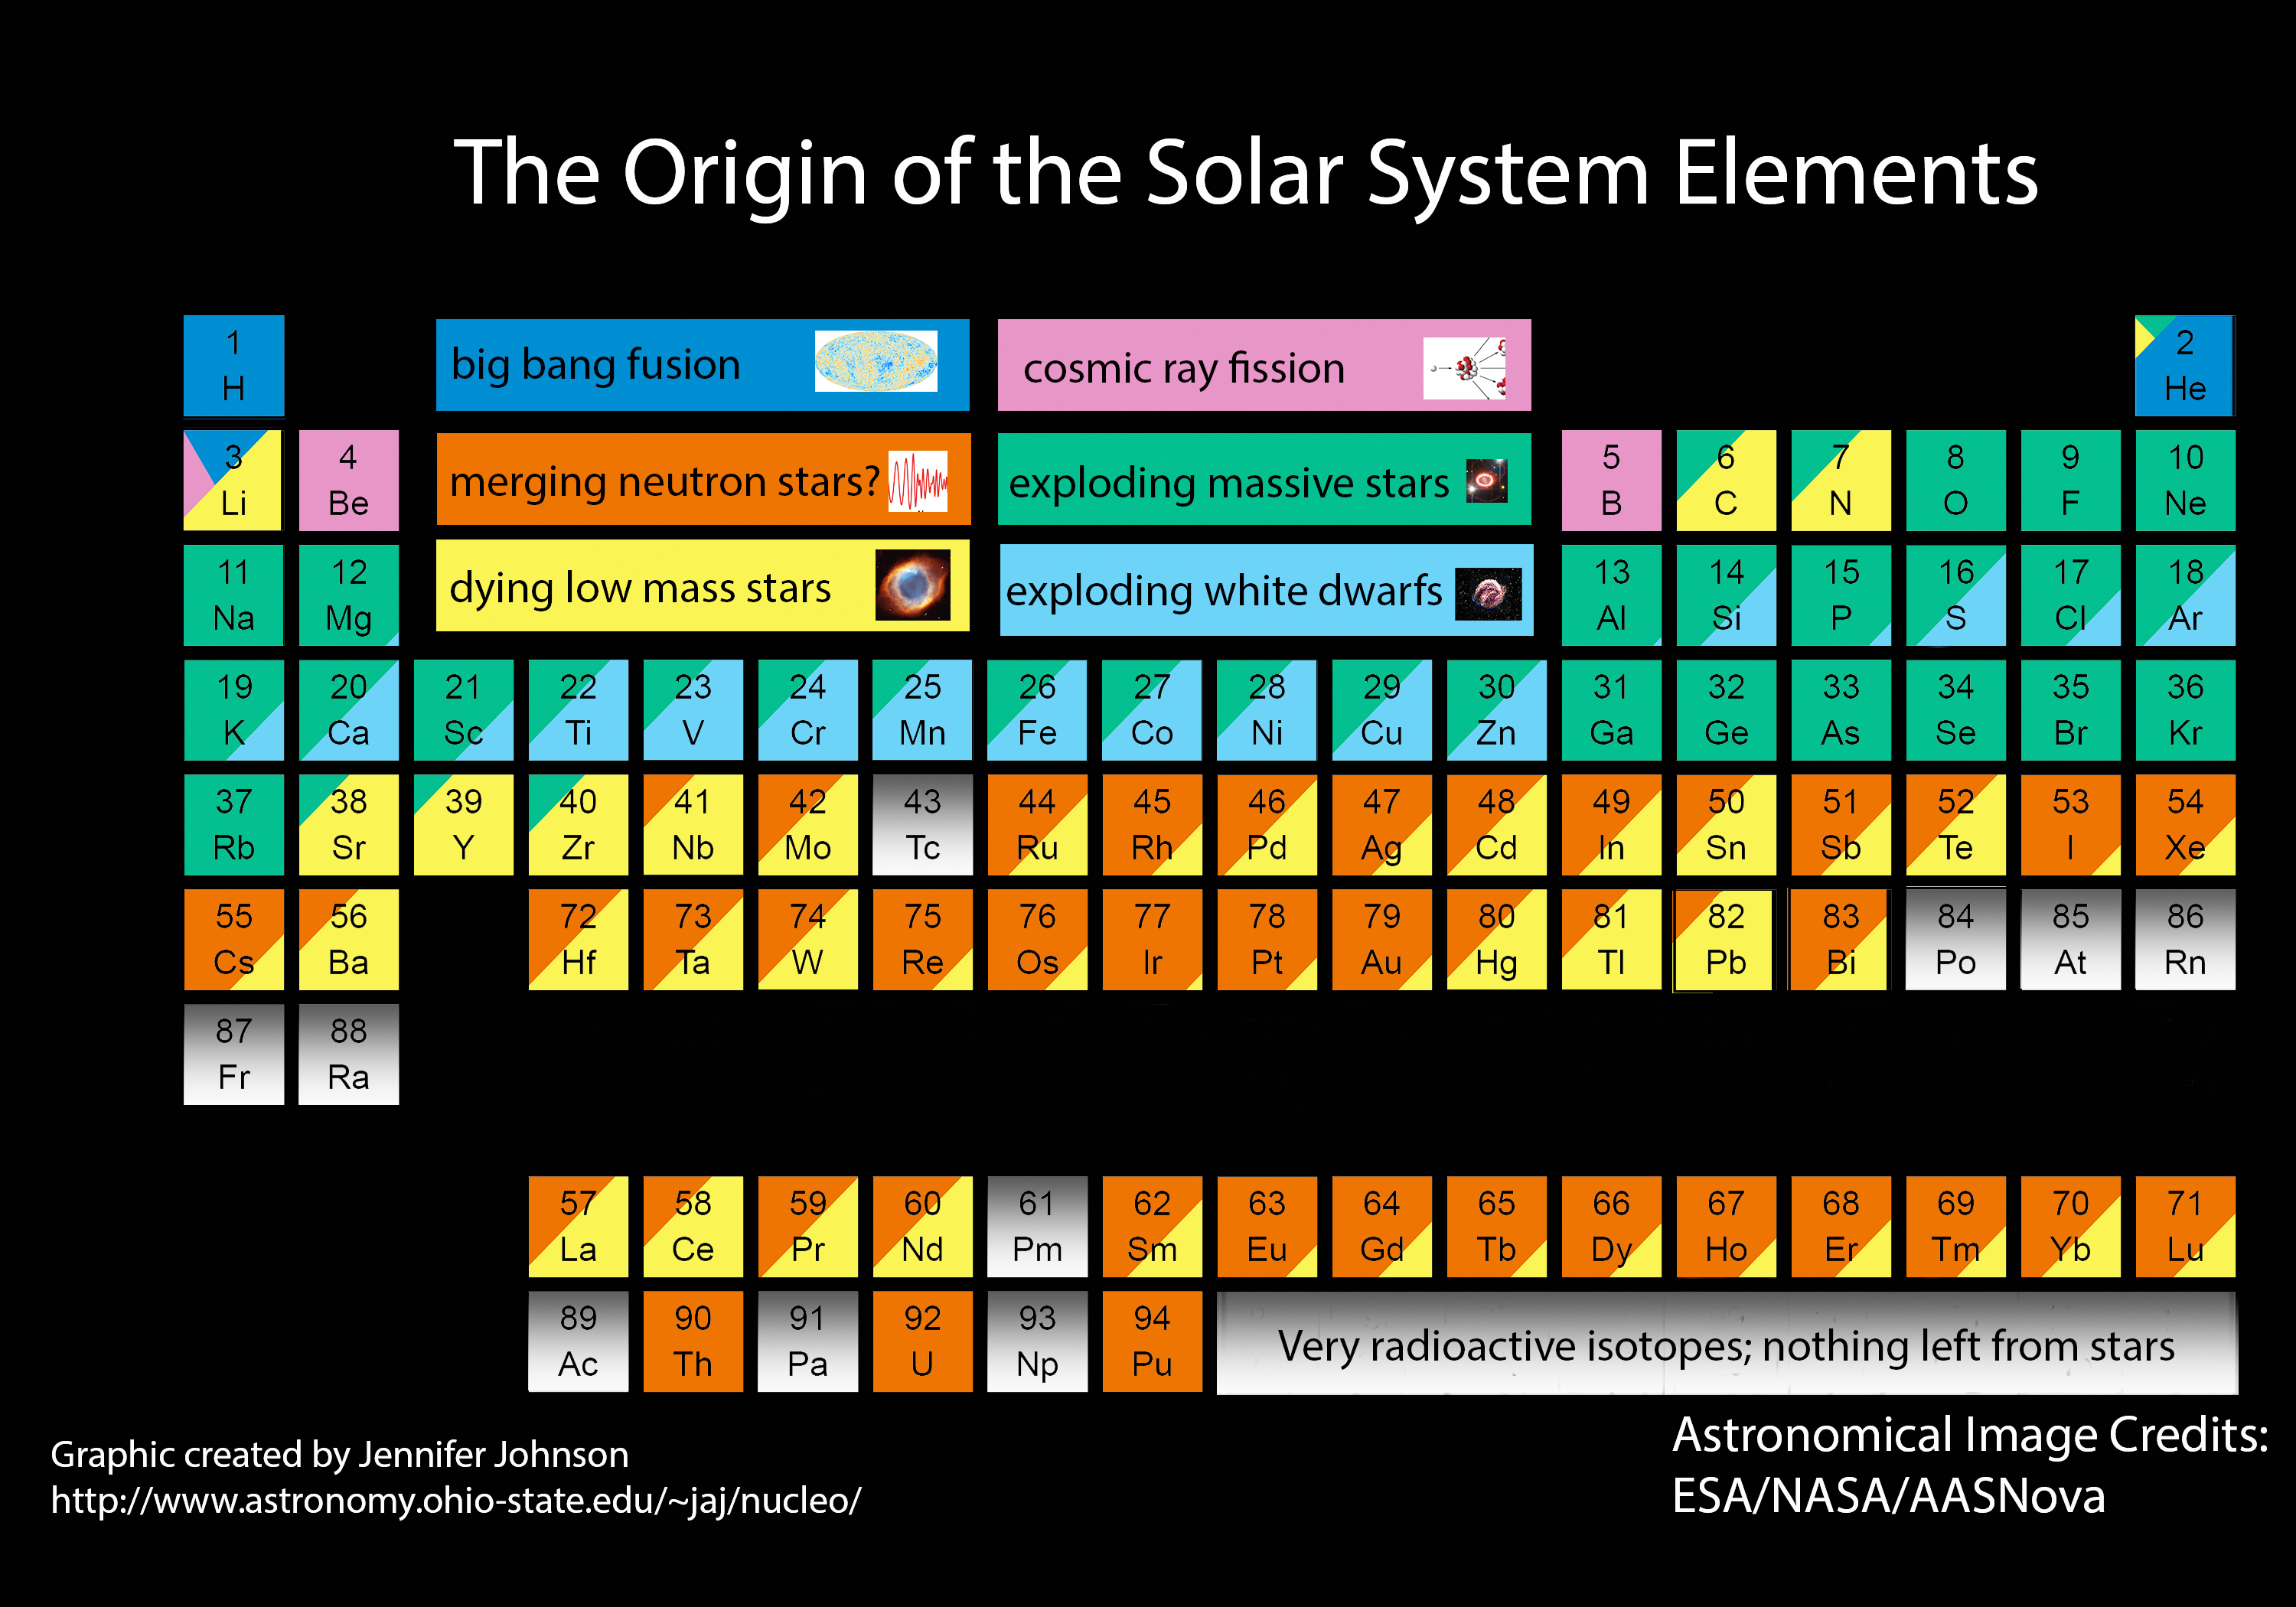
\includegraphics[width=15.75cm]{Nucleosynthesis_periodic_table_JJohnson_oct21}}
%\vspace{-0.025cm}
\caption{A compendium of current ideas on the origin of elements.}
%\medskip
\label{fig:JJsPeriodicTable}
\end{figure}


}
\end{document}

